\section*{Characteristics of thin disk oscillations}

In this section we review the characteristics of thin disk
oscillations using the dispersion relation described in the
\S \ref{sec:dispersion}. Oscillations with $m=0$ that satisfy
the dispersion relation \ref{eq:dispersion} would lead to short
wave-lengths oscillations in the disk, this oscillations are not 
interesting, since they can not be observed. Therefore the
oscillations of interest would be either \textbf{global} or
\textbf{trapped}. Global oscillations are low frequency and
one armed $m=1$. If $n=0$ they are an eccentric deformation in the
disk plane, while the $n=1$ corresponds to corrugation waves.
Trapped oscillations are present when the central object is very
massive and relativistic effects are present in the disk.
In the next subsection we describe these processes in more detail.

\subsection*{Eccentric deformations of the disk}

Eccentric dispersions corresponds to the case $m=1$ and $n=0$,
the $m = 1$ perturbations in the disk are known as one-armed
oscillations. The dispersion relation in this case is given by:

\begin{equation}
(\tilde{\omega} - \Omega)^2 - \kappa^2 = k_r^2c_s^2
\end{equation}

In the Keplerian regime and if $\tilde{\omega}$ is small and it reduces to
\verb+\citep{kato83}+:

\begin{equation}
\tilde{\omega} \sim - \dfrac{1}{2} \Omega \left( \dfrac{k_r
c_s}{\Omega}\right)^2
\end{equation}

This eccentric perturbations can be created in an homogeneous disk
if a bunch of particles with eccentric orbits at different radius.
If the disk is collisionless the perturbation with rotate with the
same period as the disk rotates, therefore the pattern would be
stationary in the rotating frame. Nevertheless collisions are present
in accretion disks, this collisions would generate a pressure that
would change the period of the one-armed perturbation. This pressure would also
make that the eccentric particles at different radii coherent. Because
the pressure restoring force is smaller that the rotation restoring
force the rotation of the distortion pattern in the rotation frame is
slow. The small frequency of this oscillations make them global.

Eccentric observations explains the violet-red (V/R) variations in
Be stars.
The negative sign tell us that the oscillations are retrograde.
This is shown in Fig.\ref{fig:vir}

\begin{figure}\label{fig:vr}
\centering
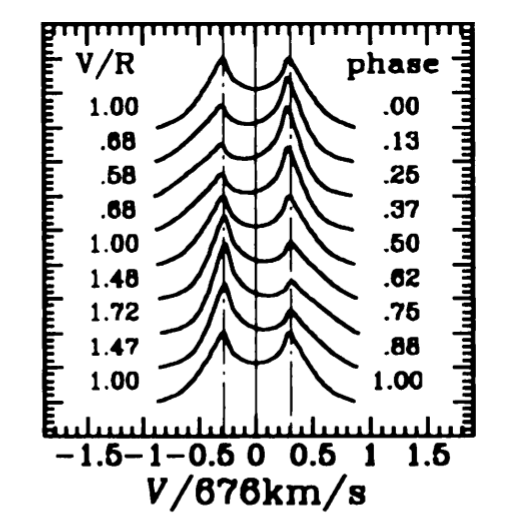
\includegraphics[scale=0.4]{VRBestars.png}
\end{figure}

\subsection*{Tidally deformed disks}


\subsection*{Low-Frequency Corrugation Waves:}

\begin{equation}
\omega \sim -\dfrac{1}{2} \Omega \dfrac{\Omega^2}{\Omega^2 -
\kappa^2} \dfrac{k_r^2 c_s^2 }{\Omega^2} + \dfrac{1}{2} \Omega
\dfrac{\Omega^2 - \Omega_{\bot}^2}{\Omega^2}
\end{equation}


\section*{Trapped Oscillations in Relativistic Disks}

\begin{figure}
\begin{subfigure}
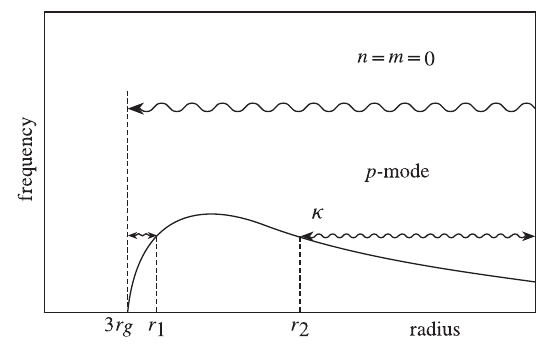
\includegraphics[scale=0.7]{rela_n0m0.png}
\end{subfigure}
\begin{subfigure}
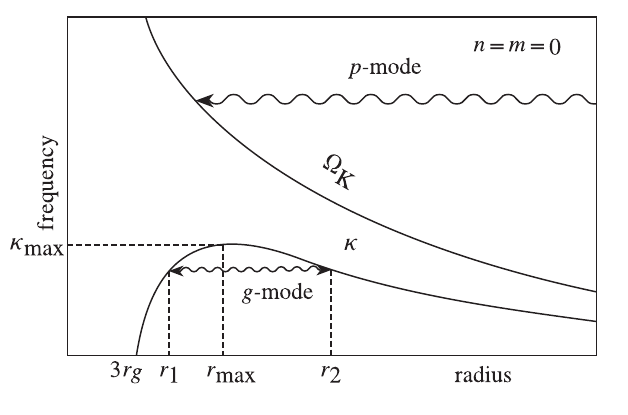
\includegraphics[scale=0.7]{rela_n1m0.png}
\end{subfigure}
\end{figure}


\subsection*{Fundamental Mode}

For the fundamental mode $n=0$ the dispersion relation reduces to:

\begin{equation}
\omega^2 = \kappa^2 + c_s^2k_r^2
\end{equation}

This is the same dispersion relation for the non-relativistic
case but $\kappa$ is different see \verb+\ref{fig:X}+.
Because $k_r > 0$ the dispersion relation implies $\omega^2 >
\kappa^2$, The region in which this is satisfied is plotted in 
\verb+\ref{fig:X2}+. The propagation regions are three which
are explained as follows, In 1 the 


